\section{Analog conception}
For the first part, let's discover the analog stuff we've done on the board.
The analog is quite absent on this board, and we only use it for two purposes :
\begin{itemize}
    \item   Get the position feedback of the servos
    \item   Monitor voltages on power rails
\end{itemize}

For the first part, we're measuring a DC voltage that move between $~0.6 \si{\volt}$
and $~2.4 \si{\volt}$. And, they're moving slowly, it take near one second to get
from one limit to the other ! For the second part, we're measuring a static DC voltage,
just to ensure the battery is present and in it's operating range.

Since the voltages are already in our measurement range, and even more, in the area
where the integrated ADC is quite linear, we don't have a lot of signal conditioning
to do.

We've only designed a filter to remove any high frequency signals that may be picked
by the wires used. Thus, we designed a Sallen-Key active filter, with a 100 Hz cutoff
frequency. This filter is absent from the power supply rail measurements, since they
are located on the PCB, and we can ensure the signal integrity with a proper layout.

The circuit is the following one :
\begin{figure}[!ht]
    \centering
    \resizebox{1\textwidth}{!}{%
    \begin{circuitikz}
    \tikzstyle{every node}=[font=\normalsize]
    \draw (5,12.25) to[european resistor,l={ \normalsize R1 = 16k$\Omega$}] (7.5,12.25);
    \draw (8.75,12.25) to[european resistor,l={ \normalsize R2 = 16k$\Omega$}] (11.25,12.25);
    \draw (15.25,12.75) node[op amp,scale=1] (opamp2) {};
    \draw (opamp2.+) to[short] (13.75,12.25);
    \draw  (opamp2.-) to[short] (13.75,13.25);
    \draw (16.45,12.75) to[short](16.75,12.75);
    \draw (12.5,12.25) to[C,l={ \normalsize C1 = 100nF}] (12.5,9.75);
    \draw (8.75,14.75) to[C,l={ \normalsize C2 = 100nF}] (11.25,14.75);
    \draw (7.5,12.25) to[short] (8.75,12.25);
    \draw (11.25,12.25) to[short] (13.75,12.25);
    \draw (8.75,14.75) to[short] (8,14.75);
    \draw (8,14.75) to[short] (8,12.25);
    \draw (11.25,14.75) to[short] (17.5,14.75);
    \draw (17.5,14.75) to[short] (17.5,12.75);
    \draw (16.75,12.75) to[short] (17.5,12.75);
    \draw (13.75,13.25) to[short] (12.5,13.25);
    \draw (12.5,13.25) to[short] (12.5,14.75);
    \node at (12.5,12.25) [circ] {};
    \node at (12.5,14.75) [circ] {};
    \draw (5,12.25) to[short, -o] (3.75,12.25) node[left] {Vin};
    \draw (17.5,12.75) to[short, -o] (18.75,12.75) node[right] {Vout};
    \draw (12.5,9.75) to (12.5,9.5) node[ground]{};
    \end{circuitikz}
    }%
    
    \label{fig:servo-filter}
    \end{figure}
\FloatBarrier

Using a SPICE simulator, we got this response :
\begin{figure}[!hbt]
    \centering
    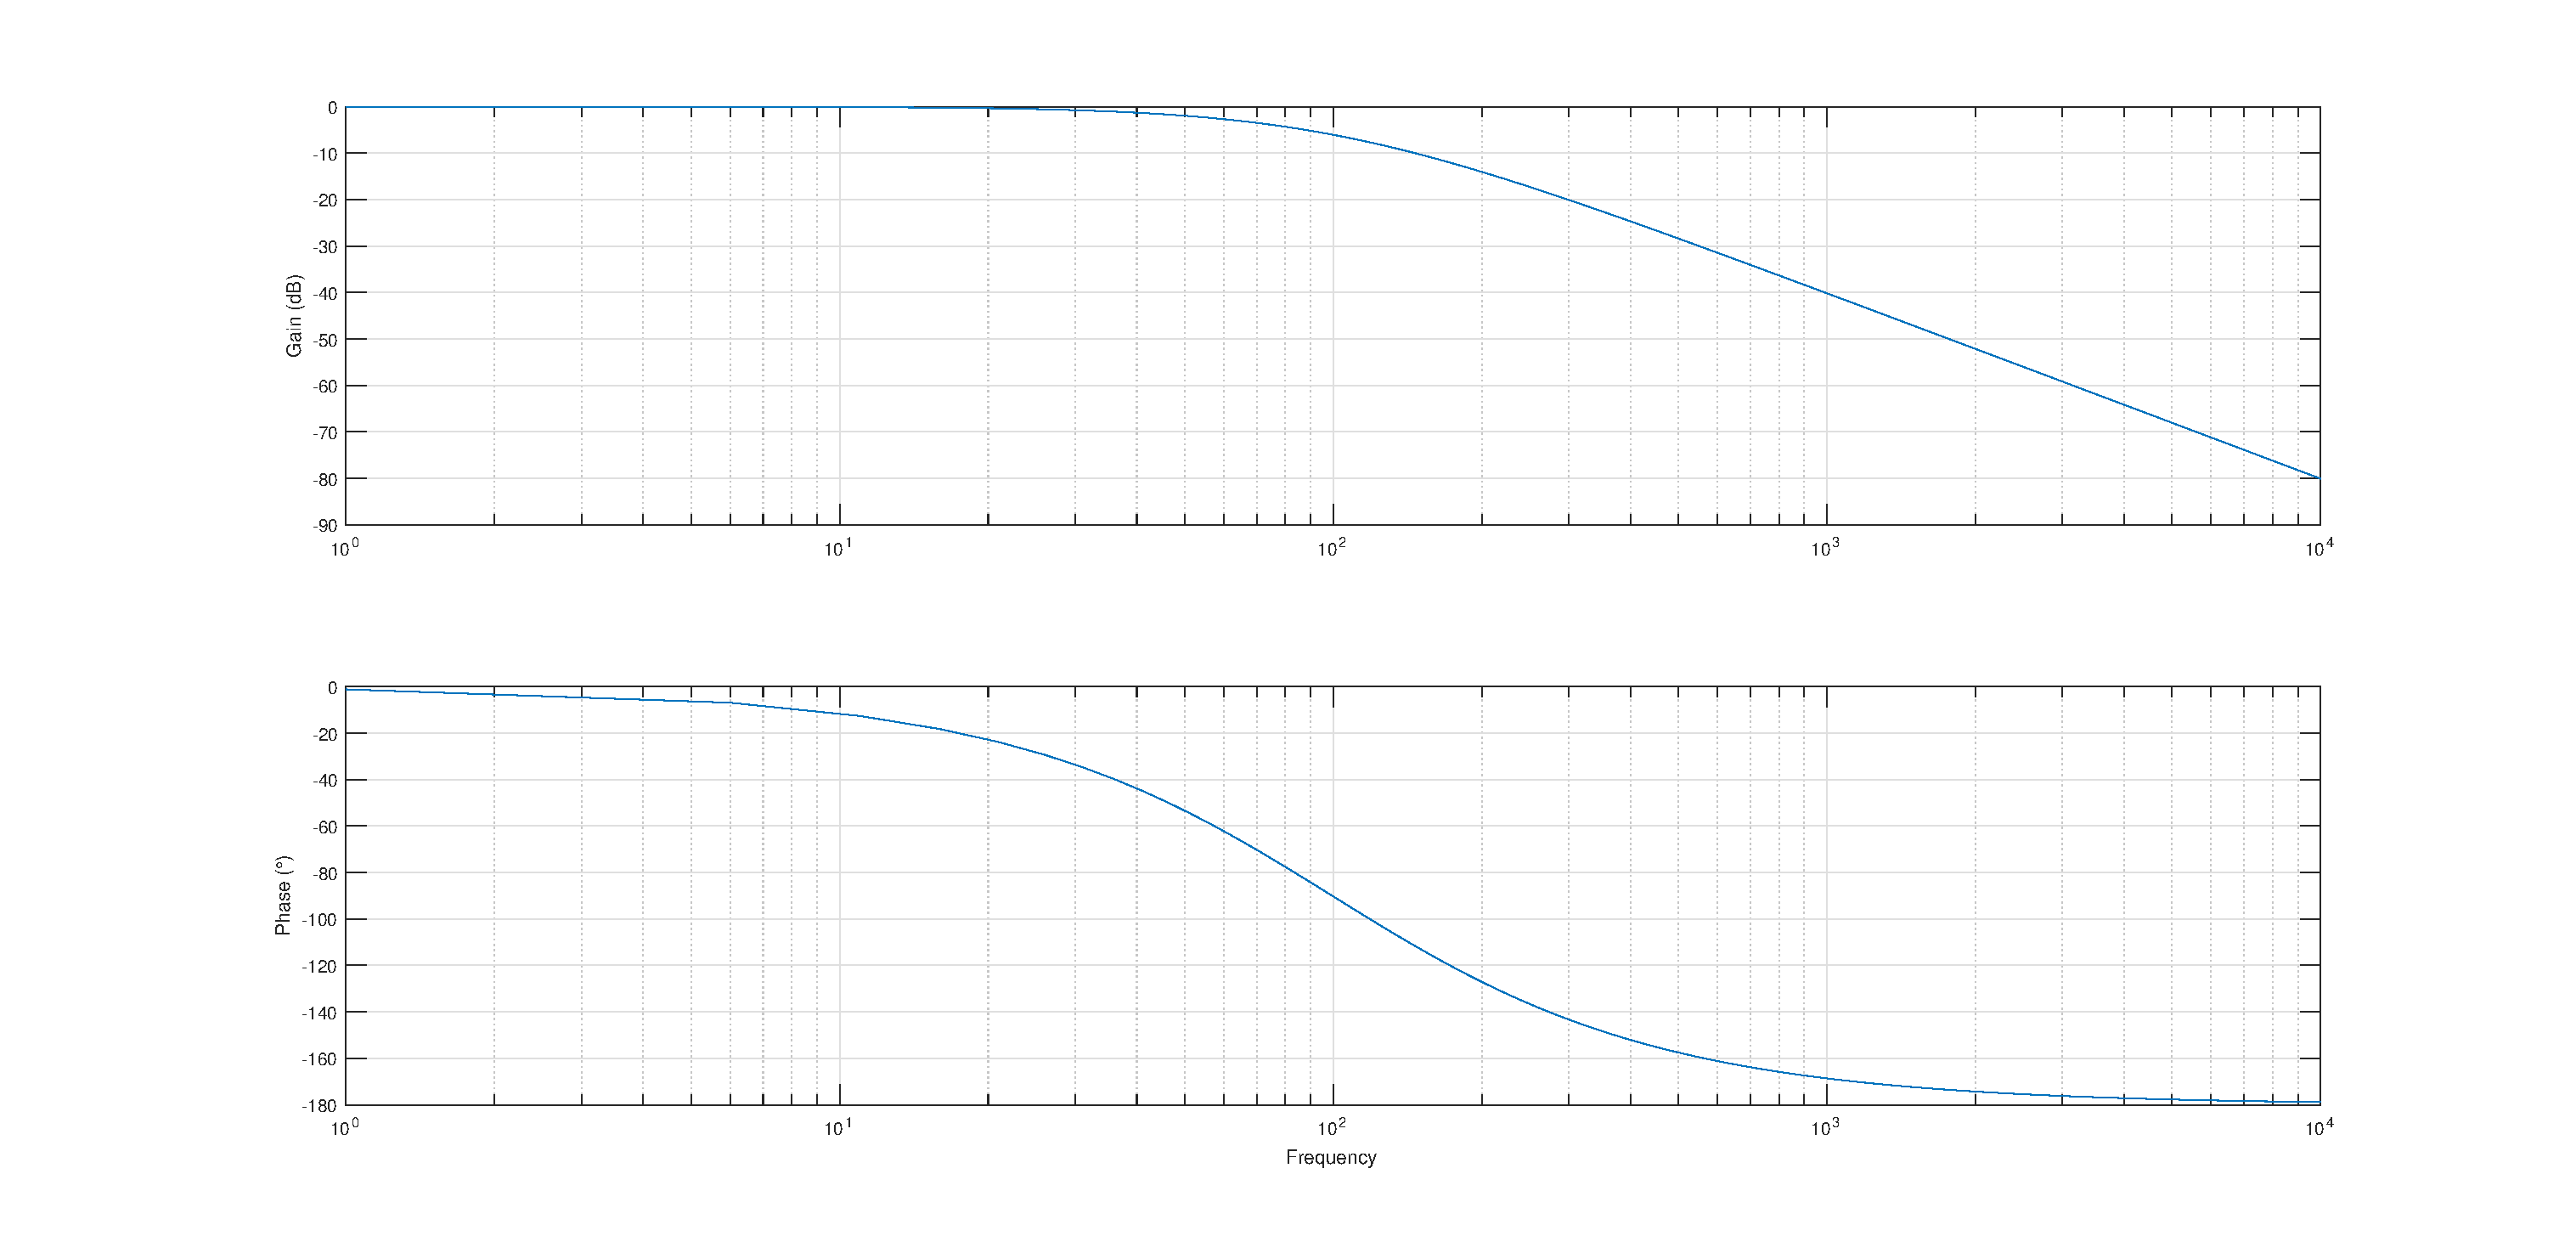
\includegraphics[width=\SchematicWidth]{\Images/Schematic/filter.eps}
    \caption{Bode plot of the filter response}
\end{figure}
\FloatBarrier

The response match our needs, which are quite simple : Remove the potential harmfull noise,
and fast variations that could occur.